\documentclass{report}
\usepackage{graphicx, amsmath, amsthm, mathtools, wrapfig, fontspec, mymacros}
\usepackage[warnings-off={mathtools-colon,mathtools-overbracket}]{unicode-math}
\setmainfont{TeX Gyre Pagella}
\setmathfont{texgyrepagella-math.otf}
\usepackage[a4paper, margin={2cm, 3cm}]{geometry}
\usepackage[fontsize=13]{scrextend}
\usepackage[font=small,skip=1pt]{caption}
\usepackage{hyperref}
\setlength\parindent{0pt}

\theoremstyle{definition}
\newtheorem{theorem}{Theorem}[chapter]

\theoremstyle{definition}
\newtheorem{definition}{Definition}[chapter]

\theoremstyle{remark}
\newtheorem*{remark}{Remark}

\newtheorem*{example}{Example}

\theoremstyle{definition}
\newtheorem{proposition}{Proposition}[chapter]

\def\eff{\ensuremath{\symcal{F}}}
\def\aii{\ensuremath{\symcal{A}}}
\def\probspace{\ensuremath{(\Omega, \eff, P)}}
\def\borel{\ensuremath{(\Omega, \eff)}}
\def\sigal{$\sigma$-algebra}
\AtBeginDocument{% to do this after unicode-math has done its work
  \renewcommand{\setminus}{\mathbin{\backslash}}%
}

\title{Probability}
\author{Salvatore Andaloro}
\date{March 2023}

\begin{document}

\maketitle
\tableofcontents
\chapter{Combinatorics}
\section{Permutations}
We have n objects, in how many ways we can pick/order them (order matters):
\begin{equation*}
    n!=n*(n-1)*(n-2)...*1
\end{equation*}
\medskip
We have n objects, but some objects are equal:
\begin{equation*}
    \frac{n!}{r_1!r_2!...}
\end{equation*}
where $r_1, r_2...$ are the number of repetitions of same objects (look at anagram example).
\section{Dispositions}
From a group n, pick k objects (order matters, we can choose each object once):
\begin{equation*}
    \frac{n!}{(n-k)!}=n*(n-1)*...*(k+1)
\end{equation*}
Example: 10 objects, 3 slots: $\#dispositions = 10*9*8 = \frac{10!}{7!}$\\
\medskip
From a group n, pick k objects (order matters, we can choose each object multiple times):
\begin{equation*}
    n^k = n*n*...*n \text{ (repeated k times)}
\end{equation*}
\section{Combinations}
From a group n, pick k objects (order doesn't matter, we can pick each object once):
\begin{equation*}
    \binom{n}{k} = \frac{n!}{k!(n-k)!}
\end{equation*}\\
\medskip
From a group n, pick k objects (order doesn't matter, we can choose each object multiple times):
\begin{equation*}
    \frac{(n+k-1)!}{k!(n-1)!}
\end{equation*}
\section{Examples}
Multiply possibilities of first case with those of second case etc.
\begin{example}
Un dipartimento di statistica decide di assegnare ai propri 25 laureati tre premi di diversa tipologia. Se ciascuno dei laureati potesse ricevere al massimo un premio, quante assegnazioni sarebbero possibili?\\
$\#E = 25*24*23$
\end{example}
\medskip
First permutate outer group, then inner group.
\begin{example}
Il Signor Amadori deve sistemare 10 libri in un ripiano della scaffalatura. Quattro libri sono di matematica, tre sono di chimica, due sono di storia e uno è di grammatica. Amadori, che è un tipo ordinato, vuole fare in modo che i libri sullo stesso argomento siano vicini in libreria. In quanti modi ciò si può realizzare?\\
$\#E = 4!*4!*3!*2!$
\end{example}
\medskip
Anagrams: $\#E = \frac{(\text{num. of letters})!}{(\text{num. of repeted letter A})!*(\text{num. of repeted letter B})!}$
\begin{example}
Quanti sono gli anagrammi di PEPPER?\\
$\#E = \frac{6!}{3!*2!}$
\end{example}
\medskip
Pick k elements in n. Order doesn't matter.
\begin{example}
Dieci ragazzi devono formare 2 squadre A e B di 5 membri ciascuna. Quante sono lo suddivisioni possibili?\\
$\#E = \binom{10}{5}=\frac{10!}{5!5!}$
\end{example}
If you have probelms asking "at least", ofter it is easier to compute the complement and then subtract.
\begin{example}
    Il sito dedicato al calcolo delle probabilità "cdp.com" richiede ai suoi utenti di registrarsi con una password. Le regole per la costruzione della password sono le seguenti:
    \begin{itemize}
        \item deve essere lunga esattamente 5 caratteri;
        \item lettere maiuscole e minuscole sono considerate distinte (la password è case sensitive);
        \item deve contenere almeno una lettera (non importa se maiuscola o minuscola) e almeno un simbolo (punto . oppure underscore);
        \item le lettere possibili sono quelle dell'alfabeto inglese (26 lettere);
        \item sono consentiti solamente lettere maiuscole o minuscole, il punto (.) e l'underscore (\_).
    \end{itemize}
    \#charachers = $26*2+2=52$\\
    From the total number of passwords($54^5$), I subtract the ones having only letters ($54^5$) and the ones having only symbols ($2^5$), so I get $n=54^4-52^5-2^5$.\\
    I can write cdp in $2^3$=8 ways. I can place cdp in 3 ways: cdp**, *cdp*, **cdp. In those 2 ** spots i can place 2 symbols ($2^2$ possibilities) or 1 symbol and 1 character ($52*2*2$ possibilities). The final result is:
    $3*2^3*(2^2+52*2^2)$ (permutations of string cdp, permutations of letters cdp, possible ways of writing **).
\end{example}
\chapter{First steps into probability}
Classical definition of probability:
\begin{equation*}
    P=\frac{\text{\#possible cases}}{\text{\#total cases}}
\end{equation*}
Only works with finite cases and equally probable cases.
\begin{definition}
An experiment is \textbf{random} if the outcome, given the initial configuration is uncertain.
\end{definition}
\begin{definition}
    $\Omega$ - \textbf{sample space}: the results, pairwise incompatible, of a random experiment.
\end{definition}
\begin{definition}
    $ \mathcal{P}(\Omega) $ - \textbf{power set} of $\Omega$: set of all subsets of $\Omega$. Cardinality is $ 2^{\#\Omega} $ (same cardinality of when we have n bits in binary (ex. if we have 4 bits then we have $2^4$ possible numbers), since we can think that 0 represents that we don't take the element, 1 if we take it).
\end{definition}
\section{Algebras and probability spaces}
\begin{definition}
    $ \mathcal{F} $ - \textbf{algebra}: family of subsets where the following holds:
    \begin{enumerate}
        \item $ \Omega \in \eff $
        \item if $ A \in \eff $ then $ A^C \in \eff $
        \item (finite case) if $ A, B \in \eff $, then $ A \cup B \in \eff $
    \end{enumerate}
\end{definition}
\vbox{
    Properties of $\eff$:
    \begin{enumerate}
        \item $\emptyset \in \eff$
        \item if $ A, B \in \eff $, then $ A \cap B \in \eff$
        \item if $ \{A_i\}^n_{i=1} \subseteq \eff$, then $\cap^n_{i=1}\, A_i \in \eff$
        \item if $A, B \in \eff $, then $A \setminus B \in \eff$
        \item if $A, B \in \eff$, then $A \,\Delta\, B \in \eff $ ($\Delta$ = elements present only in A or B, equivalent is $(A \cup B) \cap (A^C \cup B^C)$)
    \end{enumerate}
}
\begin{figure}[ht]
    \centering
    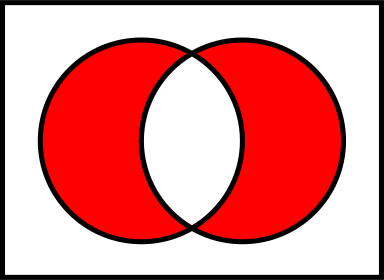
\includegraphics[width=0.25\textwidth]{images/Venn0110.png}
    \caption*{$A \,\Delta\, B$}
\end{figure}
\begin{definition}
    \sigal: same algebra as before, but also infinite unions are defined.
    Properties of \sigal s:
    \begin{enumerate}
        \item $ \Omega \in \eff $
        \item if $ A \in \eff $ then $ A^C \in \eff $
        \item for every countable family $ \{A_i\}^{+\infty}_{i=1} $ of subsets of $\Omega$, if all the sets $A_i$ are in \eff, then $\cup^{+\infty}_{i=1}\,A_i \in \eff$
    \end{enumerate}
\end{definition}
Since \sigal s accept also finite unions, all algebras are \sigal s.
\begin{example}
Difference between normal algebras and \sigal s.\\$\Omega = \symbb{N}$ $\aii$=\{$A \subseteq \symbb{N}$: $A$ is finite or $A^C$ is finite\}\\Let $A \in \aii$ and $B \in \aii$.\\If both finite, also union is finite => element of \aii. Now, let's look at numbers 2n. For any $n, 2n \in \aii$ as it is finite. But $\cup^{+\infty}_{i=1}\,2n \notin \aii$ => infinite union not contained in \aii => not a \sigal.
\end{example}
\begin{definition}
    \textbf{E - event}: every element $E \in \eff$ (\eff\, is a \sigal on $\Omega$). Singletons are elementary or atomic events.
\end{definition}
\begin{example}
    Let $\Omega=\{a, b, c\}$.\\Then we can define our \sigal{} as $\eff =\{\emptyset, \{a\}, \{b, c\}, \{a, b, c\}\}$
    \begin{itemize}
        \item $\{a\}$ is an atomic event
        \item $\{b\}$ is not an event
        \item $\{a, b, c\}$ is an event, but not atomic
    \end{itemize}
    Notice that we have checked all 3 properties of a \sigal: we have $\Omega$ and all complements.
\end{example}
\begin{definition}
    Given a set $\Omega$ and a \sigal{} \eff{}  on $\Omega$, the pair \borel{}is a \textbf{measurable space} or \textbf{Borel space}.
\end{definition}
\begin{definition}
    Given a measurable space \borel, a function $P: \eff \to \symbb{R}$ is a probability measure or probability function if it satisfies the following properties (Kolmogorov's axioms):
    \begin{enumerate}
        \item For every event E, $P(E) \ge 0$ (non negativity)
        \item $P(\Omega) = 1$ (normalization or total mass)
        \item given a countable family $\{E_i\}^{+\infty}_{i=1}$ of pairwise disjoint events, $P(\cup^{+\infty}_{i=1}E_i) = \sum_{i=1}^{\infty} P(E_i)$ ($\sigma$-additivity)
    \end{enumerate}
\end{definition}
The probability of E is the value P(E).
\begin{definition}
    Let $\Omega$ be a set, \eff{} a \sigal{} on $\Omega$, P a probability function on \eff. The triple \probspace{} is a \textbf{probability space}.
\end{definition}
Properties of probability measures:
\begin{enumerate}
    \item $P(\emptyset) = 0$
    \item if $E \in \eff \Rightarrow P(E^C) = 1 - P(E)$
    \item Let E, F events s.t. $E \subseteq F$. Then $P(E) \le P(F)$
    \item Image of any probability function is in unit interval [0, 1]
    \item \label{itm:incexl} $P(E \cup F) = P(E) + P(F) - P(E \cap F)$
    \item $P(E \cup F) \le P(E) + P(F)$
\end{enumerate}
\subsection{Inclusion-exclusion principle}
We can extend the notion of point \ref{itm:incexl} to the union of any number of sets. This is known as the inclusion-exclusion principle.
The idea is that we have to remove all elements that we have counted twice, add elements that we have removed three times etc.
\begin{figure}[ht]
    \centering
    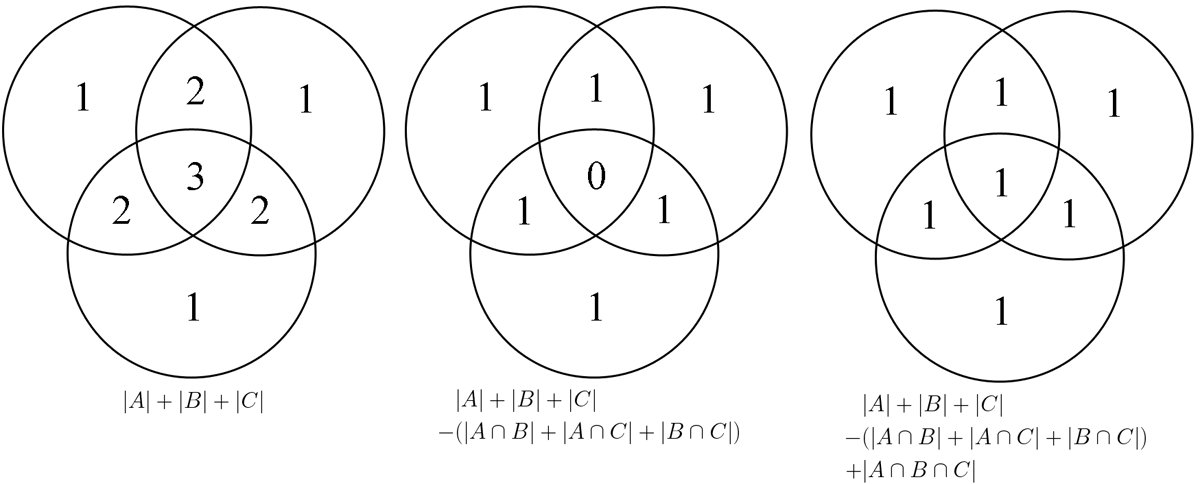
\includegraphics[width=0.8\textwidth]{images/Inclusion-exclusion-3sets.png}
    \caption*{Counting elements using the inclusion-exclusion principle with 3 sets}
\end{figure}
\begin{proposition}
    Let $\{E_i\}_{i=1}^n \subseteq \eff$  a finite family of sets. Then
    \begin{equation*}
        P\left(\bigcup_{i=1}^{n} E_i\right) = 
        \sum_{i=1}^nP(E_i) -
        \sum_{i<j}P(E_i \cap E_j) \footnote{$\sum_{i<j}=\sum_{i=1}^n\left(\sum_{j=i+1}^nP(E_i \cap E_j\right)$} +
        \sum_{i<j<k}P(E_i \cap E_j \cap E_k) +
        \cdots +
        (-1)^{n+1}P\left(\bigcap_{i=1}^nE_i\right)
    \end{equation*}
\end{proposition}
\begin{remark}
We can estimate from above (stopping at odd intersections) or below (stopping at even intersections). These are called Bonferroni bounds.
\end{remark}
\section{Conditional probability}
It is possible to extend the notion of probability spaces by adding conditions to our events.
\begin{definition}
    Given a probability space \probspace{} and two events E, F in \eff{} with $P(F) \neq 0$, we define the probability of E conditional to F ("E given F" per gli amici) as
    \begin{equation*}
        P(E|F) \coloneqq \frac{P(E \cap F)}{P(F)}
    \end{equation*}
\end{definition}
\textbf{WARNING!} $P(E|F)$ is not the same thing as $P(E \cap F)$! $P(E|F)$ denotes the probability of the intersection \underline{ONLY} on the F set, while $P(E \cap F)$ denotes the probability on the whole $\Omega$!
\begin{figure}[ht]
    \centering
    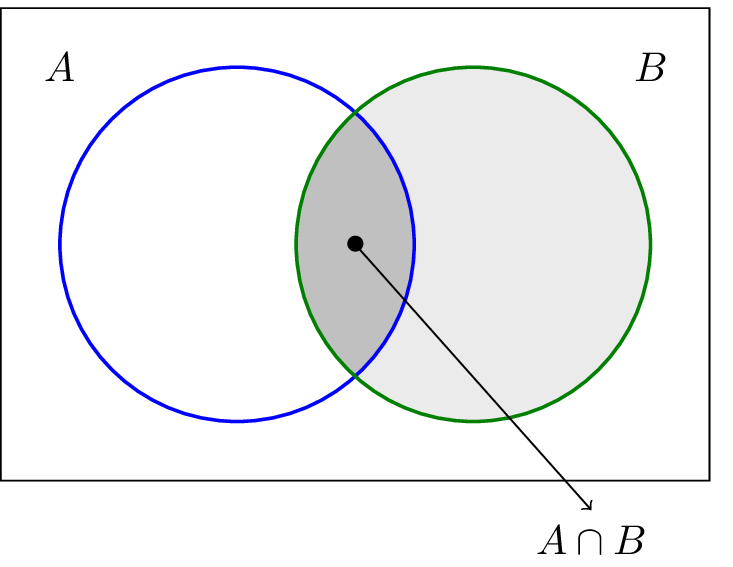
\includegraphics[width=0.4\textwidth]{images/conditional_b.png}
\end{figure}
\begin{remark}
    $P_F(\cdot) = P(\cdot{} | F) $ is a probability function, since it satisfies Kolmogorov axioms. Therefore also $P_F$ is a probability measure on the Borel space \borel, that is in general different from $P$.
\end{remark}
\begin{remark}
    Product rule
    \begin{equation*}
    \begin{gathered}
        P(E|F)=\frac{P(E \cap F)}{P(F)}\\
            \begin{aligned}
                P(E \cap F) & = P(E|F)P(F)\\
                & = P(F|E)P(E)
            \end{aligned}
    \end{gathered}
    \end{equation*}
\end{remark}
\subsection{Independence}
Let $E$ be the event that it rains tomorrow, and suppose that $P(E)=\frac{1}{3}$. Also suppose that I toss a fair coin; let $F$ be the event that it lands heads up. We have $P(F)=\frac{1}{2}$. Now I ask you, what is $P(E|F)$? What is your guess? You probably guessed that $P(E|F)=P(E)=\frac{1}{3}$. You are right! The result of my coin toss does not have anything to do with tomorrow's weather. Thus, no matter if F happens or not, the probability of E should not change. This is an example of two independent events. Two events are independent if one does not convey any information about the other.
\begin{definition}
    In a probability space \probspace{}, two events $E$, $F$ in \eff{} are \textbf{independent} (with respect to $P$) if the following holds: $P(E \cap F) = P(E) \cdot P(F)$. Sometimes the notation $E \perp F$ is used in this case.
\end{definition}
Now, let's first reconcile this definition with what we mentioned earlier, $P(E|F)=P(E)$. If two events are independent, then $P(E \cap F)=P(E)P(F)$, so
\begin{equation*}
    \begin{split}
    P(E|F) & = \frac{P(E \cap B)}{P(F)} \\
    & = \frac{P(E)P(F)}{P(F)} \\
    & = P(E).
\end{split}
\end{equation*}
An intuitive question we can ask ourselves is: is the probability of $E$ happening the same as $E$ happening after $F$? If that is the case, then the events are independent. Going back to the rain and coin case, the probability of getting heads is the same as the probability of getting heads after raining.
\begin{example}
    We have a $d6$. $E = \{2,4,6\}$ (getting an even number), $F = \{3, 6\}$ (getting a multiple of 3). Are these events independent?
    \begin{equation*}
        \frac{1}{2}\cdot\frac{1}{3} = \frac{1}{6} = P(E)P(F) = P(E \cap F) = \frac{1}{6}
    \end{equation*}
    Yes, they are. If we ask our "intuitive question", the probability of $F$ happening after $E$ is $\frac{1}{2}$, but also the probability of $E$ happening after $F$ is $\frac{1}{2}$, therefore the two events are independent.
\end{example}
Now we can of course (to be read with a with a pedantic British accent) extend this notion to more than to sets. For example, three events A, B and C are independent if all of the following conditions hold:
\begin{equation*}
    \begin{gathered}
        P(A \cap B) = P(A)P(B)\\
        P(A \cap C) = P(A)P(C)\\
        P(B \cap C) = P(B)P(C)\\
        P(A \cap B \cap C) = P(A)P(B)P(C)
    \end{gathered}
\end{equation*}
Now we can apply what we have seen with 3 sets to any number of sets.
\begin{definition}
    In a probability space \probspace, the events $E1,...,E_n$ are independent (with respect to P) if for any choice of indices (without repetition) $i_1,...,i_m$ in $\{1,...,n\}$ (with $m \le n$) it holds
    \begin{equation*}
        P\left(\bigcap_{j=1}^mE_{i_j}\right) = \prod_{j=1}^mP(E_{i_j}).
    \end{equation*}
\end{definition}
\subsection{Law of total probability/factorisation formula}
\begin{theorem}
    Let \probspace, $\{E_i\}_{i=1}^n$ disjoint, $P(E_i)>0 \; \forall i$, $\quad \bigcup_{i=1}^nE_i=\Omega$
    \begin{equation*}
        \forall E \in \eff \quad P(E) = \sum_{i=1}^n P(E \cap E_i) = \sum_{i=1}^n P(E|E_i)P(E_i)
    \end{equation*}
\end{theorem}
Using a Venn diagram, we can pictorially see the idea behind the law of total probability. In the next figure, we have
\begin{equation*}
    \begin{gathered}
    A_1 = A \cap B_1\\
    A_2 = A \cap B_2\\
    A_3 = A \cap B_3\\
    \end{gathered}
\end{equation*}
As it can be seen from the figure, $A_1$, $A_2$, and $A_3$ form a partition of the set A, and thus by the third axiom of probability
\begin{equation*}
    P(A)=P(A_1)+P(A_2)+P(A_3).
\end{equation*}
\begin{figure}[ht]
    \centering
    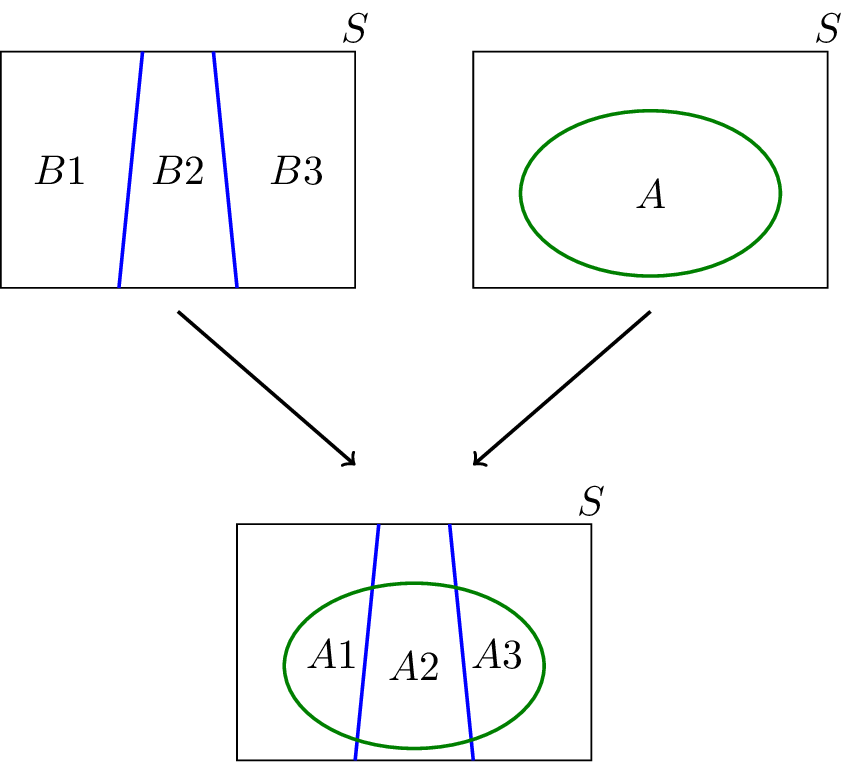
\includegraphics[width=0.5\textwidth]{images/total.png}
    \caption*{Law of total probability}
\end{figure}
\subsection{Bayes theorem}
\begin{theorem}
Let \probspace{} be a probability space and $E, F$ two events, both with non-zero probability. Then
\begin{equation*}
    P(E|F)=\frac{P(F|E)}{P(F)} \cdot P(E).
\end{equation*}
Proof:
\begin{equation*}
    P(E|F)=\frac{P(E \cap F)}{P(F)}=\frac{P(E \cap F)}{P(E)}\cdot\frac{P(E)}{P(F)}=\frac{P(F|E)\cdot P(E)}{P(F)}
\end{equation*}
\end{theorem}
\chapter{Random variables}
\begin{definition}
    In a Borel space \borel, a random variable is a function $X:\Omega \to \bbR$ s.t. for all $x \in \bbR$ the set $\{\omega \in \Omega : X(\omega) \le x\} \in \eff$.
\end{definition}

\begin{example}
    I toss a coin five times. This is a random experiment and the sample space can be written as
    \begin{equation*}
        S=\{TTTTT,TTTTH,\ldots,HHHHH\}.
    \end{equation*}
    Note that here the sample space S has $2^5=32$ elements. Suppose that in this experiment, we are interested in the number of heads. We can define a random variable X whose value is the number of observed heads. The value of X will be one of 0,1,2,3,4 or 5 depending on the outcome of the random experiment.
\end{example}
\begin{example}
    Fix $c \in \bbR\text{. } X(\omega) \equiv c \; \forall \omega \in \bbR$. $X$ is a \textbf{degenerate random variable}.
    \begin{equation*}
        \text{Pick } a \in \bbR\text{. }
        P(X=a)=\begin{cases*}
            1 & a = c\\
            0 & a \ne{} c
        \end{cases*}
    \end{equation*}
\end{example}
Not only we can check that the probability that a random variable is equal to a fixed value, but we can also check the probability that the random variable gives as results values in an interval.\\
Let's consider \probspace{} a probability space, $X:\Omega\to\bbR$ a random variable, and $A \in \calB$ ($\calB$ is a Borel \sigal{}, that is the smallest family of subsets in $\bbR$ that contains all the intervals and checks the properties of being a \sigal). Then
\begin{equation*}
    P(X \in A) = P(\{\omega \in \Omega:X(\omega)\in A\})
\end{equation*}
The function $X:\borel\to (\bbR, \calB)$ transforms the probabilities $P$ defined on the Borel space \borel{} to values in $(\bbR, \calB)$. We can denote this probability measure with $P_X$.
\begin{definition}
    Given a probability space \probspace{} and a random variable $X:\borel\to (\bbR, \calB)$, the law or \textbf{distribution} of $X$ is the probability function $P_X$ defined on $(\bbR, \calB)$ for all $A \in \calB$ as
    \begin{equation*}
        P_X(A) \coloneq P(X \in A) = P(\{\omega \in \Omega:X(\omega)\in A\})=P(X^{-1}(A))
    \end{equation*}.
\end{definition}
\begin{example}
    Let \probspace{} be a probability space, $E \in \eff$. Let's consider an urn with 50 white marbles and 50 black ones. The \textbf{indicator random variable} X tells us if $\omega$ is in the set of the event $E$ (ex. "i pick a black marble") by returning a zero or a one. Let $E$ be the event "the marble drawn is white".
    \begin{equation*}
        X = I_E(\omega)=\mathbb{1}_E(\omega)=\begin{cases*}
            1 & if $\omega \in E$\\
            0 & if $\omega \in E^C$
        \end{cases*}
    \end{equation*}
    Then for $A \in \calB$,
    \begin{equation*}
        P_X(A)=P(X \in A) = \begin{cases*}
            1 & if if $0 \in A$ and $1 \in A$\\
            \frac{1}{2} & if $0 \in A$ and $1 \notin A$\\
            \frac{1}{2} & if $0 \notin A$ and $1 \in A$\\
            0 & if $0 \notin A$ and $1 \notin A$
        \end{cases*}
    \end{equation*}
\end{example}
This tells us the following: if I choose the event $E=\text{"I pick a black marble"}$ as the indicator and a set $A$ with real numbers inside, then:
\begin{itemize}
    \item There is probability $1$ that the event happens ($1 \in A$) or doesn't happen ($0 \in A$)
    \item There is probability $\frac{1}{2}$ that the event happens ($0 \notin A \text{ and } 1 \in A$)
    \item There is probability $\frac{1}{2}$ that the event doesn't happen ($0 \in A \text{ and } 1 \notin A$)
    \item There is probability $0$ that the the random variable gives as result a number different from 0 and 1 ($0 \notin A \text{ and } 0 \notin A$)
\end{itemize}
Now we may be interested at what happens if we progressively sum the probabilities by taking a set that starts from $-\infty$ and making its right boundary vary.
\begin{definition}
    Given a random variable $X$, the \textbf{cumulative distribution function (cdf)} of $X$ is the function $F_X:\bbR\to\bbR$ defined for all $t \in \bbR$ s.t.
    \begin{equation*}
        \begin{split}
            F_X(t) & = P(X\le t)\\
            & = P_X((-\infty, t])\\
            & = P(X \in (-\infty, t])\\
            & = P(\{\omega\in\Omega:X(\omega)\le t\})
        \end{split}
    \end{equation*}
\end{definition}
\begin{figure}[ht]
    \centering
    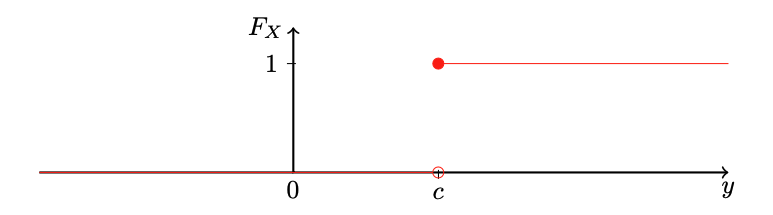
\includegraphics[width=0.6\textwidth]{images/cumulative.png}
    \caption*{Cumulative distribution function of the degenerate random variable $X\equiv c$}
\end{figure}
\begin{figure}[ht]
    \centering
    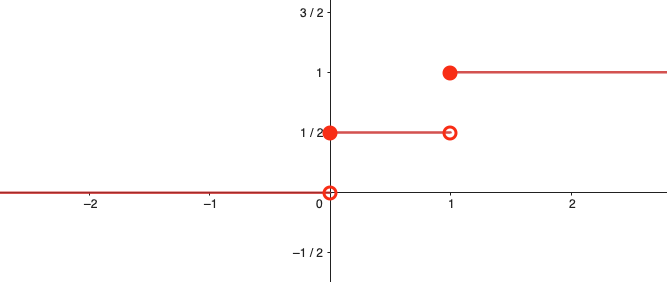
\includegraphics[width=0.61\textwidth]{images/cumulative1.png}
    \caption*{Cumulative distribution function from the marbles exercise}
\end{figure}
\vbox{
    Properties of $F_X$:
    \begin{enumerate}
        \item $F_X(\bbR) = [0, 1]$
        \item $\lim_{x \to -\infty} F_X=0, \lim_{x \to +\infty} F_X=1$
        \item non-decreasing
        \item cadlag: continuous to the right ($\lim_{x \to x_0^+} f(x) = f(x_0)$), limited to the left ($\lim_{x \to x_0^-} $ exists on $[0, 1]$)
    \end{enumerate}
}
As it can be seen from the graphs, the height of the jump at point $x_0$ represents the probability of the set of elements of $\Omega$ that have the random variable equal to $x_0$.
\section{Discrete random variables}
\begin{definition}
    A discrete random variable is a random variable returning a finite or countable number of values.
\end{definition}
\begin{remark}
    A random variable is discrete iff its distribution function is discontinuous and piecewise constant, with at most a countable number of discontinuities. These discontinuity points are the values that the random variable can take.
\end{remark}
\begin{definition}
    Let $X$ be a discrete r. v. We define the function $\rho_X:\bbR\to[0,1]$ called \textbf{probability mass function (pmf)} or absolute density of $X$ as
    \begin{equation*}
        \rho_X(k)=P(X=k)=P(\{\omega \in \Omega:X(\omega)=k\}) \; k\in\bbR.
    \end{equation*}
\end{definition}
\begin{definition}
    $\calR_X$ is the set of all the images of $X$.
    \begin{equation*}
        \calR_X=\{x \in \bbR: \rho_X(x)\ne 0\}
    \end{equation*}
\end{definition}
Properties of $\rho_X$:
\begin{enumerate}
    \item $\rho_X \in [0, 1]$
    \item $\forall x \in \calR_X^c, \rho_X(x)=0$
    \item $\sum_{x \in \calR_X}\rho_X(x)=1 $
    \item if $E \in \calB$, then $P_X(E)=\sum_{x \in \calR_X\cap E}\rho_X(x)=\sum_{x \in \calR_X}\mathbb{1}_E(x)\rho_X(x)$
    \item $F_X(t)=P_X((-\infty,t])=\sum_{x \in \calR_X}\mathbb{1}_{(-\infty, t)}(x)\rho_X(x)$
\end{enumerate}
\begin{figure}[ht]
    \centering
    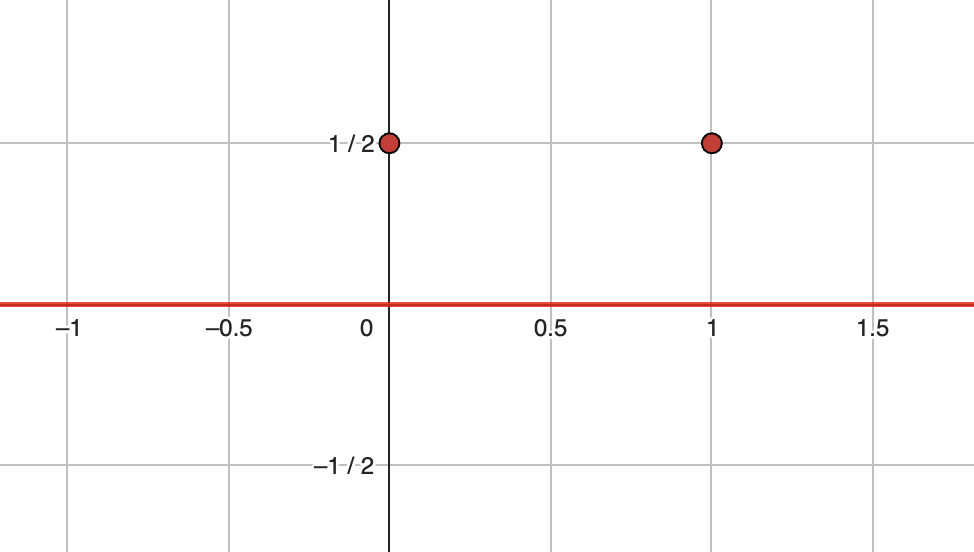
\includegraphics[width=0.6\textwidth]{images/pmf.png}
    \caption*{pmf of the marbles exercise}
\end{figure}
\section{Absolutely continuous random variables}
\begin{definition}
    A random variable $X$ is continuous if the distribution function $F_X$ is continuous. If additionally there exists a non-negative function $f_X:\bbR\to\bbR$ s.t. $\forall x\in\bbR$,
    \begin{equation*}
        F_X(x)=\int_{-\infty}^{x} f_X(y) \,dy
    \end{equation*}
    then $X$ is absolutely continuous.
\end{definition}
We can't define a probability mass function for continuous functions, because since $F_X$ is continuous (it has no jumps), for all $x \in \bbR$ we have $P(X=x)=0$ and $\rho_X$ would be 0. Instead, we can usually define the probability density function (pdf). The pdf is the density of probability rather than the probability mass. The concept is very similar to mass density in physics: its unit is probability per unit length.
\begin{definition}
    Let $X$ be an absolutely continuous random variable. By definition, there exists a non- negative function $F_X(x)=\int_{-\infty}^{x} f_X(y) \,dy$. This function $f_X$ is the probability density function (pdf), sometimes shortened to density, of $X$.
\end{definition}
\begin{remark}
    In the points where $F_X$ is differentiable, $F_X'=f(x)$.
\end{remark}
\begin{remark}
    $F_X$ can be $>1$, since it is not a probability.
\end{remark}
\newpage
\end{document}
